\chapter{Introduction}
The first chapter introduces the basic terms for structural optimization. In addition, it introduces the mathematical notation used throughout this lecture and repeats some basic concepts of tensor algebra and tensor analysis. 

\begin{objectives}{}{objectives_introduction}
After studying this chapter and finishing the exercise, you should be able to 
\begin{itemize}[label=$\dots$]
    \item distinguish three types of structural optimization problems.
    \item perform tensor algebra computations such as inner products, cross products, and outer products.
    \item employ index notation confidently.
    \item apply differential operators such as divergence and gradient on tensor fields.
\end{itemize}
\end{objectives}


\section{What is structural optimization?}
Following Gordon \cite{Gordon2003}, a \emph{structure} is "any assemblage of materials which is intended to sustain loads". The term \emph{optimization} means making things best. Thus, \emph{structural optimization} is the subject of making an assemblage of materials sustain loads in the best way \cite{Christensen2008}. 

The term \emph{best} depends on what we define to be the \emph{objective function} of our design problem. It could be the weight to obtain light structures, it could be the cost to obtain cheap structures, or it could be CO\textsubscript{2} emissions to obtain sustainable structures. Usually the optimization is subject to some \emph{constraints}, for example a certain load that has to be endured without permanent deformation. The variables that we can change to optimize the objective function are called \emph{design variables}. Depending on the choice of design variables, we generally divide three types of structural optimization problems: 
\begin{description}
    \item[Sizing optimization]{The design variables describe some technical parameters of a structure, e.g. wall thickness, diameters of holes, or the cross section of beams. We seek the optimal size of these parameters in he optimization task.}
    \item[Shape optimization]{The design variables describe the contour or boundary of a part. We seek the optimal shape of the part boundaries in the optimization task.}
    \item[Topology optimization]{The design variables describe the presence of material in a design space. We seek the optimal distribution of material within that design space.}
\end{description}

\begin{figure}[!htpb]
    \centering
    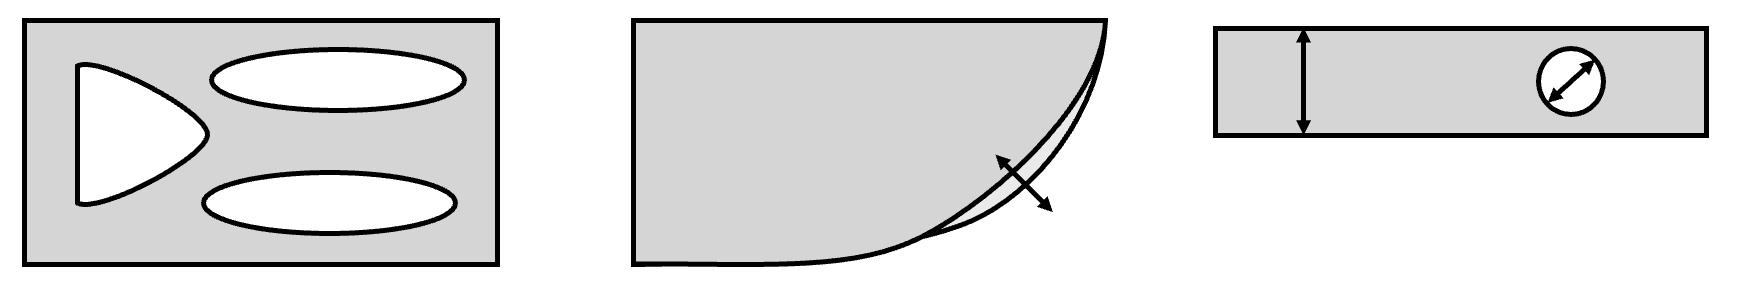
\includegraphics[width=\textwidth]{figures/structural_optimization_types.png}
    \caption{Types of structural optimization (left to right): Topology optimization, shape optimization, sizing optimization.}
    \label{fig:structural_optimization_types.}
\end{figure}

Before we can start optimizing structures, we need to recapitulate some basic tensor math, continuum mechanics and fundamentals of optimization, though. 

\section{Tensor algebra}
During this lecture we will deal with spaces, scalars, vectors, tensors, matrices and other mathematical objects. To support understanding of which objects are used in each context, we introduce some notation rules. 

\subsection{Scalars}
A scalar variable, such as a temperature, has no direction and is completely described by a single real value. Scalars are denoted as variables in regular font, for example
\begin{equation}
    a \in \mathcal{R}.
\end{equation}

\subsection{Vectors}
Most objects have some sort of direction associated to it (e.g. a velocity or a force). They are defined in a \emph{vector space} 
$\mathcal{R}^d$, where $d$ is the dimension of the vector space. A \emph{vector} is an element of the vector space that fulfills so-called vector axioms and is denoted with lowercase letters in bold font, e.g. 
\begin{equation}
    \textbf{a} \in \mathcal{R}^d.
\end{equation}
In order to describe components of a vector, it is convenient to define a \emph{basis}. A basis is given by a subset of vectors ${\mathbf{e}_1,\mathbf{e}_2,...,\mathbf{e}_d}$ that are linearly independent and span the entire vector space.
More specifically, we use an orthonormal basis (\emph{ONB}) that is spanned by normalized and orthogonal vectors $\{\mathbf{e}_i\}$. The orthogonality is expressed as  
\begin{equation}
    \label{eq:orthogonality}
    \mathbf{e}_i \cdot \mathbf{e}_j = \delta_{ij}
\end{equation}
with the \emph{Kronecker symbol} 
\begin{equation}
    \delta_{ij} = 
    \begin{cases}
    1 & \text{if }  i=j \\
    0 & \text{else}.
    \end{cases}
\end{equation}

\begin{example}{Standard basis in 3D Euclidean space}{basis_example}
    The standard basis for the three-dimensional ($d=3$) Euclidean space is given by the set of three vectors
    \begin{equation}
        \{\mathbf{e}_1=(1,0,0), \mathbf{e}_2=(0,1,0), \mathbf{e}_3=(0,0,1)\}.
    \end{equation}
\end{example}

With a basis, we can define a vector in terms of \emph{coordinates} $(a_1, a_2, ..., a_d)$ as 
\begin{equation}
    \label{eq:coordinates}
    \mathbf{a} = \sum_i a_i \mathbf{e}_i. 
\end{equation}
It is important to note that these coordinates depend on the basis. The same vector $\mathbf{a}$ may be expressed with coordinates $(a_1, a_2, ..., a_d)$ for a basis $\{\mathbf{e}_i\}$ and $(\tilde{a}_1, \tilde{a}_2, ..., \tilde{a}_d)$ for a basis $\{\tilde{\mathbf{e}}_i\}$. 

%It is a bit cumbersome to write the summation sign all the time. Therefore, we apply \emph{Einstein's summation convention} or \emph{index notation}: We omit the summation sign, but keep in mind that if two equal indices appear in an expression, then we sum over that index. Therefore the expressions
%\begin{equation}
%    \mathbf{a} \Leftrightarrow \sum_i a_i \mathbf{e}_i \Leftrightarrow a_i \mathbf{e}_i \Leftrightarrow a_i
%\end{equation}
%are equivalent, where the last expression $a_i$ omitted the basis assuming that it is the standard basis.

We define the \emph{inner product} or \emph{scalar product} of two vectors $\mathbf{a}, \mathbf{b} \in \mathcal{R}^d \rightarrow \mathcal{R}$ as 
\begin{equation}
    \mathbf{a} \cdot \mathbf{b} 
        = \sum_i a_i \mathbf{e}_i \cdot \sum_j b_j \mathbf{e}_j 
        =  \sum_{i,j} a_i b_j \overbracket{(\mathbf{e}_i \cdot \mathbf{e}_j)}^{\delta_{ij}} 
        = \sum_{i,j} a_i b_j \delta_{ij} = \sum_{i} a_i b_i
\end{equation}
using Equation \eqref{eq:orthogonality}.
There are two remarks at this point: First, the result of the scalar product between two vectors is a scalar as it is just a summation of coordinates. Second, the Kronecker symbol can be interpreted as an operator that replaces an index.

\begin{example}{Calculations with the Kronecker symbol}{kronecker}
    These are a couple of examples for Kronecker computations: 
    \begin{align}
        \delta_{11}     &= 1\\
        a \delta_{33}   &= a \\
        \sum_i \delta_{ii} &= d 
    \end{align}
\end{example}

The cross product between two vectors results in a vector perpendicular to the first two vectors and a magnitude equal to the area spanned by the two vectors. It can be denoted for two vectors $\mathbf{a},\mathbf{b} \in \mathcal{R}^3 \rightarrow \mathcal{R}^3$ as 
\begin{equation}
    \mathbf{a} \times \mathbf{b} = \sum_i \epsilon_{ijk} a_j b_k \mathbf{e}_i 
\end{equation}
with the permutation symbol 
\begin{equation}
    \epsilon_{ijk} = 
    \begin{cases}
        +1  & \text{if } (ijk) \text{ is an even permutation of } (1,2,3)\\
        -1  & \text{if } (ijk) \text{ is an odd permutation of } (1,2,3)\\
        0   & \text{else}.
    \end{cases}
\end{equation}

\subsection{Tensors}
Vectors are not sufficient to describe all directional objects needed in this lecture. A stress, for example, results in a traction vector that also depends on the cutting plane defined by its normal direction. 
% following the Lemma of Cauchy 
% \begin{equation}
%     \mathbf{t} = \pmb{\sigma} \mathbf{n} = \sigma_{ij} n_j \mathbf{e}_i.
% \end{equation}
In a sense, the stress tensor combines two directions and we learn in basic mechanics courses that one index is attributed to the direction and one to the plane. We can also think about the stress tensor as a mapping from one vector to another vector or as a multi-dimensional array containing the values of $S_{ij}$.

Such \emph{tensor} objects can be constructed by the \emph{outer product}, \emph{tensor product}, or \emph{dyadic product} of two vectors $\mathbf{a}, \mathbf{b} \in \mathcal{R}^d \rightarrow \mathcal{R}^{d \times d}$ as 
\begin{equation}
    \label{eq:tensorproduct}
    \mathbf{a} \otimes \mathbf{b} = \sum_{i,j} a_i b_j \mathbf{e}_i \otimes \mathbf{e}_j,
\end{equation}
where the term $\mathbf{e}_i \otimes \mathbf{e}_j$ may be interpreted as a new basis for the tensor. We may also specify such a tensor $\mathbf{A} \in \mathcal{R}^{d \times d}$ directly as 
\begin{equation}
    \mathbf{A} = \sum_{i,j} A_{ij} \mathbf{e}_i \otimes \mathbf{e}_j ,
\end{equation}
where bold capital letters are used primarily for such tensors.
The entries of these tensors may be interpreted as two-dimensional arrays
\begin{equation}
    \mathbf{a} \otimes \mathbf{b} =
    \begin{pmatrix}
         a_1 b_1    & a_1 b_2   & \dots   & a_1 b_d  \\
         a_2 b_1    & a_2 b_2   & \dots   & a_2 b_d  \\
         \dots      & \dots     & \dots   & \dots  \\
         a_d b_1    & a_d b_2   & \dots   & a_d b_d  \\
    \end{pmatrix}_{\{\mathbf{e}_i\}}
\end{equation}
and 
\begin{equation}
    \mathbf{A} =
    \begin{pmatrix}
         A_{11}    & A_{12}   & \dots   & A_{1d}  \\
         A_{21}    & A_{22}   & \dots   & A_{2d}  \\
         \dots      & \dots     & \dots   & \dots  \\
         A_{d1}    & A_{d2}   & \dots   & A_{dd}  \\
    \end{pmatrix}_{\{\mathbf{e}_i\}}
\end{equation}
for this specific ONB. Again, note that these entries could be different in a different basis.

In fact, we can interpret some objects of the previous chapter as tensors. A vector is a first-order tensor 
\begin{equation}
    \mathbf{a} = \sum_{i} a_i \mathbf{e}_i = 
    \begin{pmatrix}
         a_1 \\
         a_2 \\
         \dots \\
         a_d
    \end{pmatrix}_{\{\mathbf{e}_i\}}
\end{equation}
and the Kronecker symbol can be used to define a second-order unit tensor 
\begin{equation}
    \pmb{I} = \sum_{i,j} \delta_{ij} \mathbf{e}_i \otimes \mathbf{e}_j = 
    \begin{pmatrix}
         1      & 0     & \dots & 0 \\
         0      & 1     & \dots & 0 \\
         \dots  & \dots & \dots & \dots  \\
         0      & 0     & \dots & 1  \\
    \end{pmatrix}_{\{\mathbf{e}_i\}}
\end{equation}
using a bold capital letter for the second-order tensor, and the permutation symbol is a third-order tensor with a three-dimensional array specifying its entries: 
\begin{equation}
    \pmb{\epsilon} = \sum_{i,j,k} \epsilon_{ijk} \mathbf{e}_i \otimes \mathbf{e}_j \otimes \mathbf{e}_k = \sum_{i,j,k}
    \vcenter{\hbox{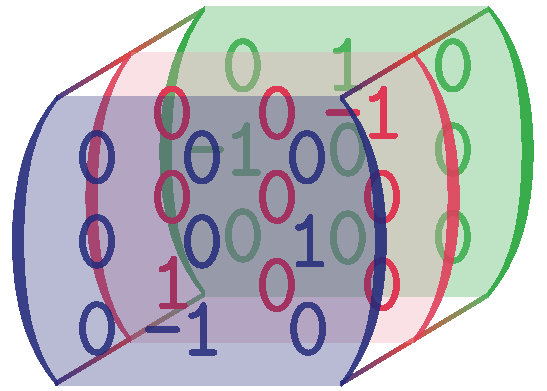
\includegraphics[width=0.2\textwidth]{figures/epsilontensor.pdf}}}
    \quad 
    \mathbf{e}_i \otimes \mathbf{e}_j \otimes \mathbf{e}_k
\end{equation}

We may extend this concept further to higher orders. A stiffness tensor for example maps a second-order strain tensor to a second-order stress tensor and thus it is a fourth-order tensor, which we denote with double-stroke capital letters. More general, a fourth order tensor may be obtained by an outer product of two second-order tensors $\mathbf{A},\mathbf{B}\in \mathcal{R}^{d \times d} \rightarrow \mathcal{R}^{d \times d \times d \times d}$ as 
\begin{equation}
    \mathbb{C} = \mathbf{A} \otimes \mathbf{B} = \sum_{i,j,k,l} A_{ij}B_{kl}  \mathbf{e}_i \otimes \mathbf{e}_j \otimes \mathbf{e}_k \otimes \mathbf{e}_l.
\end{equation}

We define the tensor contraction of two second-order tensors $\mathbf{A},\mathbf{B} \in \mathcal{R}^{d \times d} \rightarrow \mathcal{R}^{d \times d}$: 
\begin{align}
    \mathbf{A} \cdot \mathbf{B} 
        &= \sum_{i,j} A_{ij} \mathbf{e}_i \otimes \mathbf{e}_j \cdot \sum_{k,l}B_{kl} \mathbf{e}_k \otimes \mathbf{e}_l \\
        &= \sum_{i,j,k,l} A_{ij} B_{kl} (\mathbf{e}_i \otimes \overbracket{\mathbf{e}_j) \cdot  (\mathbf{e}_k}^{\delta_{jk}} \otimes \mathbf{e}_l) \\
        &= \sum_{i,j,k,l} A_{ij} B_{kl} (\overbracket{\mathbf{e}_j \cdot  \mathbf{e}_k}^{\delta_{jk}}) \mathbf{e}_i \otimes \mathbf{e}_l \\
        &= \sum_{i,j,k,l} A_{ij}B_{kl} \delta_{jk} \mathbf{e}_i \otimes \mathbf{e}_l \\
        &= \sum_{i,j,l} A_{ij}B_{jl} \mathbf{e}_i \otimes \mathbf{e}_l
\end{align}
Essentially, this contracts the inner dimensions. This is an exemplary summary of such contractions:

\begin{example}{Tensor contraction}{tensorcontractionexample}
    Contraction of two first order tensors $\mathbf{a},\mathbf{b} \in \mathcal{R}^d \rightarrow \mathcal{R}$: 
    \begin{equation}
        \mathbf{a} \cdot \mathbf{b} = \sum_i a_i b_i 
    \end{equation}
    Contraction of two second-order tensors $\mathbf{A},\mathbf{B} \in \mathcal{R}^{d \times d} \rightarrow \cdot \mathcal{R}^{d \times d}$: 
    \begin{equation}
        \mathbf{A} \cdot \mathbf{B} = \sum_{i,j,k} A_{ij} B_{jk} \mathbf{e}_i \otimes \mathbf{e}_k
    \end{equation}
    Contraction of a second-order tensor $\mathbf{A} \in \mathcal{R}^{d \times d}$ and a first-order tensor $\mathbf{b} \in \mathcal{R}^d \rightarrow \mathcal{R}^d$: 
    \begin{equation}
        \mathbf{A} \cdot \mathbf{b} = \sum_{i,j} A_{ij} b_j \mathbf{e}_i 
    \end{equation}
\end{example}

We can apply the inner product multiple times. For example, we can define the double contraction of two second-order tensors $\mathbf{A},\mathbf{B} \in \mathcal{R}^{d \times d} \rightarrow \mathcal{R}$: 
\begin{align}
    \mathbf{A} : \mathbf{B} 
        &= \sum_{i,j} A_{ij} \mathbf{e}_i \otimes \mathbf{e}_j :  \sum_{k,l} B_{kl} \mathbf{e}_k \otimes \mathbf{e}_l \\
        &= \sum_{i,j,k,l} A_{ij}B_{kl} (\underbracket{\mathbf{e}_i \otimes \overbracket{\mathbf{e}_j) :  (\mathbf{e}_k}^{\delta_{jk}} \otimes \mathbf{e}_l}_{\delta_{il}}) \\
        &= \sum_{i,j,k,l} A_{ij}B_{kl} \delta_{jk} \delta_{il} \\
        &= \sum_{i,j} A_{ij}B_{ji}
\end{align}

Essentially, the number of dots in the product indicates how many dimensions we want to contract.

\begin{example}{Tensor double contraction}{tensordoublecontractionexample}
    Double contraction of two second-order tensors $\mathbf{A},\mathbf{B} \in \mathcal{R}^{d \times d} \rightarrow \mathcal{R}$: 
    \begin{equation}
        \mathbf{A} : \mathbf{B} = \sum_{i,j} A_{ij} B_{ji} 
    \end{equation}
    Double contraction of two fourth-order tensors $\mathbb{A},\mathbb{B} \in \mathcal{R}^{d \times d \times d \times d} \rightarrow \mathcal{R}^{d \times d \times d \times d}$: 
    \begin{equation}
        \mathbb{A} : \mathbb{B} = \sum_{i,j,k,l,m,n} A_{ijkl} B_{lkmn} \mathbf{e}_i \otimes \mathbf{e}_j \otimes \mathbf{e}_m \otimes \mathbf{e}_n
    \end{equation}
    Double contraction of a fourth-order tensor $\mathbb{A} \in \mathcal{R}^{d \times d \times d \times d}$ and a second-order tensor $\mathbf{B} \in \mathcal{R}^{d \times d} \rightarrow \mathcal{R}^{d \times d}$: 
    \begin{equation}
        \mathbb{A} : \mathbf{B} = \sum_{i,j,k,l} A_{ijkl} B_{lk} \mathbf{e}_i \otimes \mathbf{e}_j
    \end{equation}
\end{example}

Finally, we denote the trace, transposition and inverse of a tensor as $\text{tr}(\mathbf{A})$, $\mathbf{A}^\top$, and $\mathbf{A}^{-1}$, respectively.

\section{Tensor analysis}
In many physical processes, variables appear as \emph{tensor fields} with a dependency on a spatial variable $\mathbf{x} \in \mathcal{R}^d$. Some examples are given here:
\begin{example}{Tensor fields}{tensorfieldexample}
    A temperature field is a scalar field
    \begin{equation}
        \theta: \mathcal{R}^d \rightarrow \mathcal{R}.
    \end{equation}
    A displacement field is a vector field
    \begin{equation}
        \mathbf{u}: \mathcal{R}^d \rightarrow \mathcal{R}^d.
    \end{equation}
    A stress field is a second-order tensor field
    \begin{equation}
        \mathbf{S}: \mathcal{R}^d \rightarrow \mathcal{R}^{d \times d}.
    \end{equation}
\end{example}

In most governing equations of physical processes, we need to compute differential operations on these fields. Therefore, the following sections introduce the most important differential operators for tensor fields assuming that the fields are differentiable and that we are using Cartesian coordinates \footnote{In curvilinear coordinates things get a bit more complicated. We stick to Cartesian coordinated in this lecture. }. 

A common notation for differential operations on tensor fields utilizes the Nabla operator 
\begin{equation}
    \nabla = \sum_i \frac{\partial }{\partial x_i} \mathbf{e}_i = 
    \begin{pmatrix}
            \frac{\partial}{\partial x_1} \\
            \frac{\partial}{\partial x_2} \\
            \dots \\
            \frac{\partial}{\partial x_d} \\
        \end{pmatrix}_{\{\mathbf{e}_i\}}
\end{equation}
The Nabla operator may be interpreted as a first-order tensor or vector, which upon multiplication in an inner product or cross product applies a derivative instead of being just multiplied. 

\subsection{Gradient}
The gradient computes the partial derivative with respect to each spatial direction and represents this information as a higher-order tensor. We denote the gradient operator $\nabla (\bullet)$. The resulting tensor is increased by one order as shown in the following examples:
\begin{example}{Gradient}{gradientsexample}
    Gradient of a scalar field
    \begin{equation}
        \nabla \theta = \sum_i \frac{\partial \theta}{\partial x_i} \mathbf{e}_i =
        \begin{pmatrix}
            \frac{\partial \theta}{\partial x_1} \\
            \frac{\partial \theta}{\partial x_2} \\
            \dots \\
            \frac{\partial \theta}{\partial x_d} \\
        \end{pmatrix}_{\{\mathbf{e}_i\}}
    \end{equation}
    Gradient of a vector field
    \begin{equation}
        \nabla \mathbf{u} = \sum_{i,j} \frac{\partial u_i}{\partial x_j} \mathbf{e}_i \otimes \mathbf{e}_j
        = 
        \begin{pmatrix}
            \frac{\partial u_1}{\partial x_1} & \frac{\partial u_1}{\partial x_2} & \dots & \frac{\partial u_1}{\partial x_d}\\
            \frac{\partial u_2}{\partial x_1} & \frac{\partial u_2}{\partial x_2} & \dots & \frac{\partial u_2}{\partial x_d}\\
            \dots & \dots & \dots & \dots\\
            \frac{\partial u_d}{\partial x_1} & \frac{\partial u_d}{\partial x_2} & \dots & \frac{\partial u_d}{\partial x_d}\\
        \end{pmatrix}_{\{\mathbf{e}_i\}}
    \end{equation}
\end{example}

The gradient may be interpreted as a measure for how much a tensor changes in each direction. 

We may compute the gradient of a gradient of a scalar field. If all the partial derivatives exits, we call the entries a \emph{Hessian}.

\begin{example}{Hessian}{hessianexample}
    Hessian of a scalar field
    \begin{equation}
        \nabla^2 \theta = \sum_{i,j} \frac{\partial^2 \theta}{\partial x_i \partial x_j} \mathbf{e}_i \otimes \mathbf{e}_j
        = 
        \begin{pmatrix}
            \frac{\partial^2 \theta}{\partial x_1 \partial x_1} & \frac{\partial^2 \theta}{\partial x_1 \partial x_2} & \dots & \frac{\partial^2 \theta}{\partial x_1 \partial x_d}\\
            \frac{\partial^2 \theta}{\partial x_2 \partial x_1} & \frac{\partial^2 \theta}{\partial x_2 \partial x_2} & \dots & \frac{\partial^2 \theta}{\partial x_2 \partial x_d}\\
            \dots & \dots & \dots & \dots\\
            \frac{\partial^2 \theta}{\partial x_d \partial x_1} & \frac{\partial^2 \theta}{\partial x_d \partial x_2} & \dots & \frac{\partial^2 \theta}{\partial x_d \partial x_d}\\
        \end{pmatrix}_{\{\mathbf{e}_i\}}
    \end{equation}
\end{example}

\subsection{Divergence}
The divergence computes the partial derivative with respect to each spatial direction, sums these values up and represents this information as a lower-order tensor. We denote the divergence operator $\nabla \cdot (\bullet)$. The resulting tensor is increased by one order as shown in the following examples:
\begin{example}{Divergence}{divergenceexample}
    Divergence of a vector field
    \begin{equation}
        \nabla \cdot \mathbf{u} =  \sum_i \frac{\partial u_i}{\partial x_i}
        = 
        \frac{\partial u_1}{\partial x_1} + \frac{\partial u_2}{\partial x_2} + \dots + \frac{\partial u_d}{\partial x_d}
    \end{equation}
    Divergence of a second-order tensor field
    \begin{equation}
        \nabla \cdot \mathbf{S} = \sum_{i,j} \frac{\partial S_{ij}}{\partial x_j} \mathbf{e}_i
        = 
        \begin{pmatrix}
            \frac{\partial S_{11}}{\partial x_1} + \frac{\partial S_{12}}{\partial x_2} + \frac{\partial S_{13}}{\partial x_3} \\
            \frac{\partial S_{21}}{\partial x_1} + \frac{\partial S_{22}}{\partial x_2} + \frac{\partial S_{23}}{\partial x_3}\\
            \frac{\partial S_{31}}{\partial x_1} + \frac{\partial S_{32}}{\partial x_2} + \frac{\partial S_{33}}{\partial x_3}
        \end{pmatrix}_{\{\mathbf{e}_i\}}
    \end{equation}
\end{example}

The divergence may be interpreted as the tensor field's source. If the divergence is positive, this is a source and if it is negative, it will act as a sink. 

\bibliographystyle{unsrtnat}
\bibliography{literature} 

% SEE https://biomechanics.stanford.edu/me337/me337_s02.pdf